% !TEX encoding = UTF-8 Unicode
% !TEX root = ../../Masterthesis.tex

\chapter{Introduction}\label{ch:introduction}

When setting out to write this thesis it was with the purpose to understand modern film scoring. The question I was asking myself was in the lines of: ``What is going on with modern film music? This does not sound like it used to!'' What I was trying to formulate back then was that I had noticed a change of focus in film music of today, i.e. how composers now choose to ``talk'' to the audience. My theory was that film music was moving away from the strong concept of melody given to us with \textit{John Williams} and \textit{Star Wars}, to make room for texture: Enormous walls of sound featuring huge orchestras with lots and lots of synths and sound effects. This made me think that perhaps the new \textit{leitmotif} was texture. My wanderings aside however, the scope of a single thesis is not enough to cover such an extensive topic. But, one must start some place and I landed on figuring out how film music has evolved. To further narrow it down I chose to study \textit{science fiction}, specifically the music of \textit{Star Trek}. Star Trek is a special case in movie history. It has been running since 1969 in one form or another. The first movie came out in 1979 and the last one in 2013. It is ideal to use as a case tracking its evolution over time. The most available material to conduct research on is the Star Trek motion pictures. All of the scores has been released as special edition CD's containing most cues from the motion pictures, making it easy to focus on the music. I will discuss Star Trek in depth in chapter \ref{ch:star trek}.

\begin{figure}
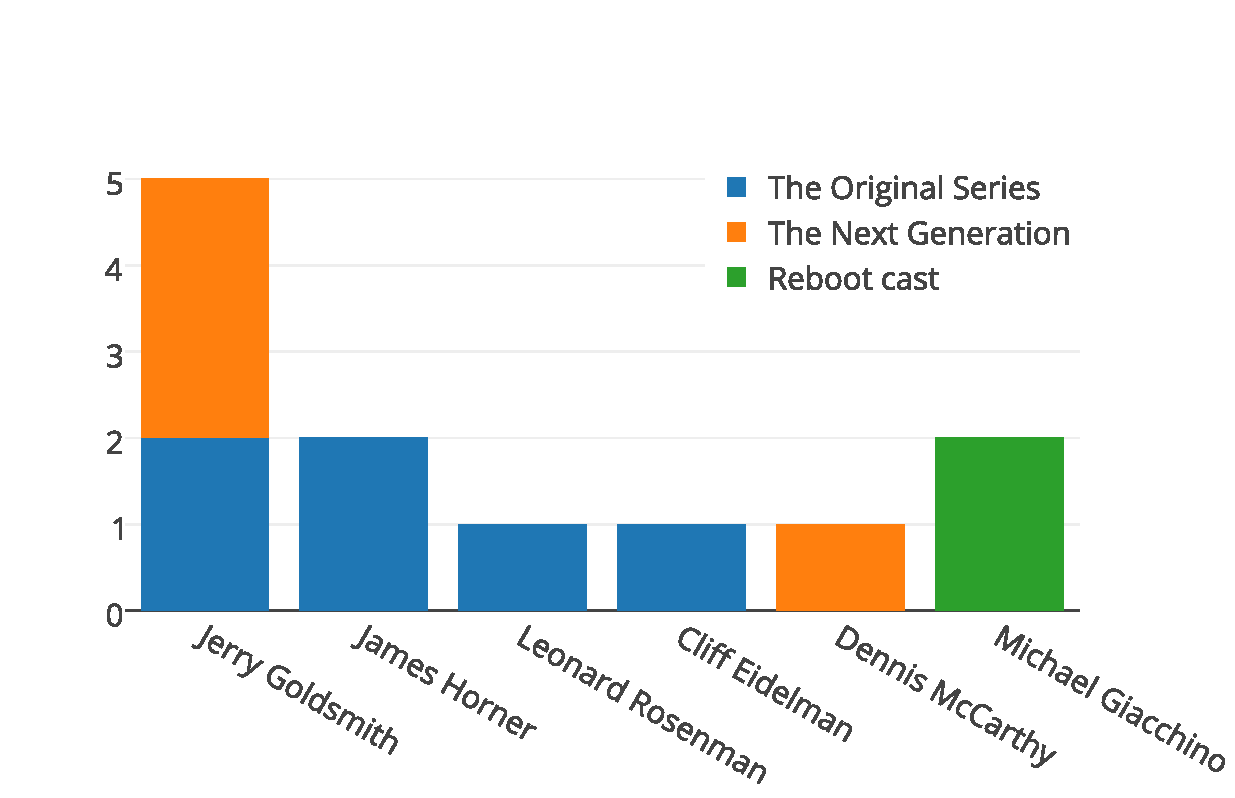
\includegraphics[width=\linewidth]{star_trek_composers_and_movies}
	\caption{Star Trek composers and movies}
	\label{fg:st composers}
	\setfloatalignment{b}
\end{figure}

But even so, there are no official scores to procure. I was able to get in touch with people able to help me get a look at the actual scores used during the different recording sessions, but that meant traveling to Hollywood and Paramount studios. By the time I had gotten this information any window to apply for funding was past. Therefore I chose to transcribe the music myself. One challenge of transcribing music this detailed is the amount of time required transcribing the examples. With twelve movies to chose from the question regarding what I was going to focus on arose. Star Trek, the movies is divided into three epochs: The Original Series, The Next Generation and the Reboot. I thought it best to choose two movies from each epoch. One composer in the Star Trek universe stands out: \textit{Jerry Goldsmith}. He has scored five of the twelve movies during a timespan of 23 year making him part of the quintessential \textit{sound} of Star Trek. The choice fell on the two first films, \textbf{''The Motion Picture''}, by Goldsmith and \textbf{''The Wrath of Kahn''}, by \textit{James Horner}. Both critically acclaimed for their music. The next obvious candidates was the newest films from the reboot series: \textbf{''Star Trek''} and \textbf{''Into Darkness''} featuring composer \textit{Michael Giacchino}. What to chose from ``The Next Generation'' era was harder. I wanted to study how the music has evolved over time therefore looking for some sort of continuity. The choice fell on Goldsmiths scores for \textbf{''First Contact''} and \textbf{''Nemesis''}. I present my analysis in chapter \ref{ch:sttmp} through \ref{ch:into_darkness}. That being said, the other scores are well worth the attention and should be included in a later research. A table containing the complete list of Star Trek movies can be found on page \pageref{tb:filmography} and the complete list of all composers associated with the Star Trek universe can be found on page \pageref{tb:star trek composers}.

\marginnote{
\textbf{The filmography in question:
}
\begin{itemize}
\item The Motion Picture, \textit{1979}, TOS
\item The Wrath of Kahn, \textit{1982}, TOS
\item First Contact, \textit{1996}, TNG
\item Nemesis, \textit{2002}, TNG
\item Star Trek, \textit{2009}, Reboot
\item Into Darkness, \textit{2013}, Reboot
\end{itemize}
}

Now my quest was crystalizing, I wanted to study the musical conventions of Star Trek. How to go about it? My formal training is for the most part traditional so the analytical tools I already knew was not ideal to handle the diverse tonality of movie scores. I knew ``Hollywoodian'' movie scores since \textit{Erich Wolfgang Korngold} and \textit{John Williams} had their roots in nineteen century classical music, also know as the romantic period of classical music. \textit{Romantic} music is mostly tonal, meaning it uses major and minor chords and scales to build the tonality, but it is not necessarily functional. By that I mean progressions build upon the \textit{circle of fifths} and the famous \(I-IV-V^{7}-I\). This brings us to the idea of a \textit{tonic}, a tonal ``home'' where we feel at peace after pursuing the chord furthest away from the tonic, the \textit{dominant}. It would be wrong to say that romantic music does not utilize the idea of a tonic, but it was not a concept expanded upon as they did in the classical era. Instead they had what I call \textit{tonal centers}. These are focal point for any given progression and stands as the root of origin. This differentiation is necessary because harmonic progressions can be made with a different logic than that of the circle of fifths. There are plenty of analytic tools to chose from when working with functional music and atonal music but I was having a hard time finding the right tool for non-unified tonal music.

During my research I came upon Frank Lehman's dissertation on \textit{''Reading Tonality Through Film: Transformational Hermeneutics and the Music of Hollywood'' (2012)}. His research was focusing on \textit{neo-Riemannian Theory}, a theory made to address the analytical challenges nineteen century music presented, applied to film music. I will discuss the application and execution of this theory in chapter \ref{ch:nrt}. To further explain how my analysis is constructed, I will discuss music analysis in general in chapter \ref{ch:musical analysis}. 

To aid the reader in analytic process I have chosen to include the transcriptions immediately following the corresponding analysis. The analytic legend will be discussed on page \pageref{fg:analysis legend} and finally I will present my conclusions in chapter \ref{ch:the musical conventions}.

As a final note I want to talk about what I am not covering in this thesis. First of all, I have chosen to use musical terms and notation to explain my findings. This means the reader will have to have a fairly advanced understanding of musical theory to fully appreciate the content of this thesis. I will not talk about film music history in general: How the film music traditions has evolved from live music to Korngold to Steiner to Williams and even Zimmer is extremely interesting, but it is covered to such an extent elsewhere there simply is no point including it and secondly, I do not believe being reminded of this knowledge will have an impact on the understanding of the main topic of this thesis. My goal is that the content of this thesis provides ample understanding of the main analysis and that the reader will come to appreciate the inner workings of the music in question and how it has evolved.

% Revidert jan 2016
